\documentclass[11pt,english]{article}
\usepackage[T1]{fontenc}
\usepackage{babel}
\usepackage{graphicx}



\title{Working with Streaming Data:\\Analysis of Twitter Tweets}

\author{
	Anand Raghuraman\\
	\texttt{anand.raghuraman@wsu.edu}
	\and
	Ehdieh Khaledian\\
	\texttt{ehdieh.khaledian@wsu.edu}
}

\begin{document}
	
\maketitle{}

\begin{abstract}
As more data is generated, it is becoming increasingly important to be able to work with real-time
data. In this project twitter streaming API is used to capture three different tweets. Then, captured
tweets are analyzed using Python and R to find how much people are happy in each U.S. state,
which celebrity from “Breaking Bad” series is the happiest one and word frequency in tweets.
\end{abstract}

\section{Introduction}
Social networks today has become a very popular communication tool among Internet users.
Millions of messages are appearing daily in popular web-sites that provide services for
microblogging such as Twitter1, Tumblr2, Facebook3. Authors of those messages write about their
life, share opinions on variety of topics and discuss current issues. Because of a free format of
messages and an easy accessibility of microblogging platforms, Internet users tend to shift from
traditional communication tools (such as traditional blogs or mailing lists) to this services. As more
and more users post about products and services they use, or express their political and religious
views, these web-sites become valuable sources of people’s opinions and sentiments. Such data
can be efficiently used for marketing or social studies.
Furthermore, as more data is generated, it’s becoming increasingly important to be able to work
with real-time data and being able to work with streaming data is become a critical skill for any
aspiring data scientist. Real-time, or streaming, data is generated continuously, and in the case of
the stock market, there can be millions of rows generated every hour. Due to size and time
constraints, there often isn’t a neat dataset that you can analyze and we’ll need to either store the
data to analyze later, or analyze it in real time, as you get it. It means, we are not dealing with
historical data anymore.
In this project, we fetch the real-time data from twitter to analyze. In Twitter, everyday very large
number of very short messages create by the users. The contents of the messages vary from 
personal thoughts to public statements. Therefore, a lot of information can be obtained from twitter
as their users post everyday what they like/dislike, and their opinions on many aspects of their life.
The list of different ways to use Twitter could be long, and with 50 million of tweets per day, there
is a lot of data to analyze and to play with.
To work with twitter’s data, Twitter Streaming API, gives developers and data scientists access to
multiple types of streams (public, user, site), with the difference that the streaming API collects
data in real-time as opposed to the search API, which retrieves past tweets. Public streams are
streams of public data that flow through twitter. We can use this for following specific users or
topics, and for data mining. User streams contain data corresponding to a single user’s stream.
Lastly, site streams are multi-user version of the user stream.

\section{Problem Definition}
Sentiment analysis over Twitter offer organizations, politician, and social developers a fast and
effective way to monitor the publics’ feelings towards their decision, brand, business, directors,
etc. In this project, we apply Sentiment analysis on fetched tweets to find a tweet that is most
positive or negative. In this case, we use the positive and negative scores of each tweet to find the
happiest and unhappiest people. It can be used for other purposes like approval and disapproval of
people about a new decision, person, brand, movie, etc.

\section{Algorithms}
We have split the entire project into four parts namely\\1)Fetching tweets.\\2)Finding the frequency of each term in the tweets\\3)Sentimental Analysis on the tweets.\\4)Analyzing the happiest actors in breaking bad tv series\\ 5)Finding out the top 5 happiest states.

\subsection{Fetching Tweets}
Algorithm 1 is used for fetching tweets. We have used Twitter API in order to fetch the tweets.

\subsection{Computing the frequency of different terms}
We have used the Tweets that have been fetched and computed frequency of the terms using the formula:
[number of occurrences of the term in all tweets]/[number of occurrences of all terms in all tweets]

\subsection{Sentimental analysis}
Algorithm 3 will compute the sentiment of each tweet based on the sentiment scores of the
terms in the tweet. The sentiment of a tweet is equivalent to the sum of the sentiment scores for
each term in the tweet.\\ \\
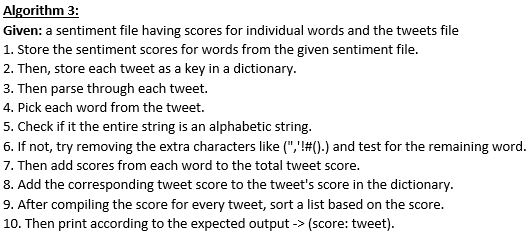
\includegraphics{algo3.jpg}

\subsection{Analyzing the happiest actor}
Algorithm 4 is used to find out the happiest actor in breaking bad TV series.\\
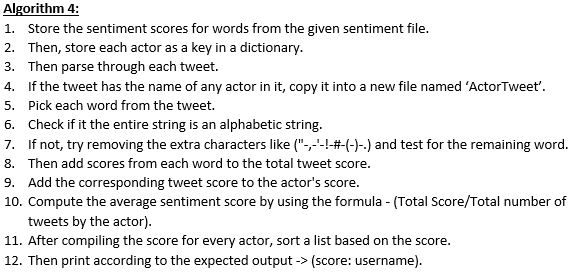
\includegraphics{algo4.jpg}

\subsection{Analysing the top happiest and unhappiest states}
Algorithm 5 is used to find out the top happiest and unhappiest states in the US.\\
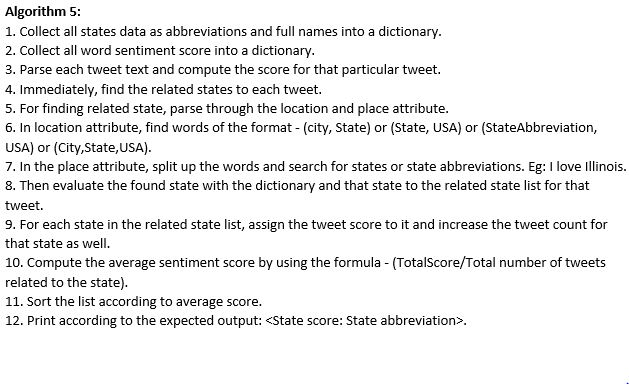
\includegraphics{algo5.jpg}


\section{Implementation}
The Dataset for this project is derived from live twitter feeds using Twitter's Streaming API.The Streaming APIs give developers low latency access to Twitter’s global stream of Tweet data. A proper implementation of a streaming client will be pushed messages indicating Tweets and other events have occurred, without any of the overhead associated with polling a REST endpoint.Connecting to the streaming API requires keeping a persistent HTTP connection open.\\
Figure 4.1 gives a schematic representation of the process:\\
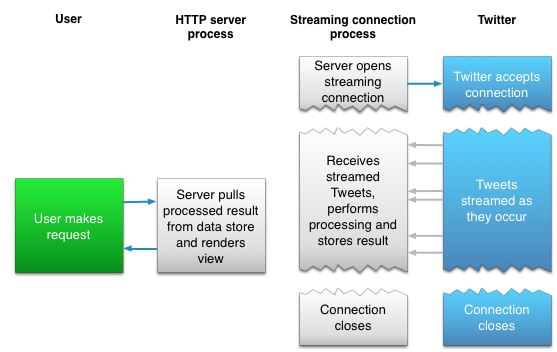
\includegraphics{fig4-2.jpg}\\ \\
The streaming process gets the input Tweets and performs any parsing, filtering, and/or aggregation needed before storing the result to a data store. The HTTP handling process queries the data store for results in response to user requests.\\ \\
Our Analysis had three different parts.So, we used three different types of data from the tweet file we derived from the API.\\ \\
For the first part, we used the entire data in order to compute the term frequency.Using the algorithm stated above, we were able to compute the term frequency. For finding out the happiest and unhappiest actors in the breaking bad TV series, we had to use only part of the dataset that was relevant for the analysis and thus had to first store the required data from the dataset into a separate file and then use the algorithms stated above to perform the analysis.For the last part of the project in which we found the happiest and unhappiest states in US, we did the a similar process as we had done for finding the happiest actors.In addition to these data we had used two datasets, one of which had the list of all stopwords and another which had the list of sentiment scores for individual words.




\end{document}
